%!TEX root = ../thesis.tex
%*******************************************************************************
%*********************************** First Chapter *****************************
%*******************************************************************************

\chapter{Introduction \label{cha:Into}}  %Title of the First Chapter

\ifpdf
    \graphicspath{{Chapter1/Figs/Raster/}{Chapter1/Figs/PDF/}{Chapter1/Figs/}}
\else
    \graphicspath{{Chapter1/Figs/Vector/}{Chapter1/Figs/}}
\fi


%********************************** %First Section  **************************************

\nomenclature[z-EO]{EO}{Earth Observation.}
\nomenclature[z-SAR]{SAR}{Synthetic Aperture Radar.}
\nomenclature[z-CESM]{CESM}{Community Earth System Model.}
\nomenclature[z-NCAR]{NCAR}{National Centre for Atmospheric Research.}
\nomenclature[z-FDA]{FDA}{Functional Data Analysis.}
\nomenclature[a-t]{t}{Temporal location.}
\nomenclature[a-s]{$\ve{s}$}{Spatial location.}
\nomenclature[a-T]{$\mathcal{T}$}{Temporal domain.}
\nomenclature[a-S]{$\mathcal{S}$}{Spatial domain.}
\nomenclature[a-X]{$\mathcal{X}$}{Functional random variable.}
\nomenclature[a-N]{N}{Number of spatial observations.}
\nomenclature[a-Ji]{$J_i$}{Number of temporal observations for $i^\text{th}$ functional observation.}
\nomenclature[a-y]{$y_{ij}$}{Observed response at time $t_j$ for $i^\text{th}$ functional observation.}
\nomenclature[a-Y]{Y}{Observed data set.}
\nomenclature[g-chi]{$\chi$}{Functional data (observation of $\mathcal{X}$).}
\nomenclature[g-epsilon]{$\varepsilon_{ij}$}{Noise process at time $t_j$ for $i^\text{th}$ functional observation.}
\nomenclature[s-i]{$i$}{Spatial index.}
\nomenclature[s-j]{$j$}{Temporal index.}


\section{Earth Observation\label{sec:eo}}
Many areas of science produce data on both a spatial and temporal scale.
Take for example, the production of Earth Observation data. Earth Observation (EO) is the collection of information on the state of a physical, chemical or biological system of the planet.
Typically EO data is acquired through some form of remote sensing in addition to perhaps some in-situ measurements.
EO data is acquired to study a process either over a large area of land, a large time horizon, or both.
For example, such EO studies include; land usage change in wetland environments in southern Spain, \citep{muro_short-term_2016}, crop production in the Netherlands, \citep{khabbazan_crop_2019}, and land deformation of the Tuscany region over a two year time period, \citep{raspini_continuous_2018}.
In each case there is significant spatial and temporal dependency that is to be considered in the observed processes.
For example, \citeauthor{raspini_continuous_2018} use the temporal dependency in ground deformation signals to highlight areas of significant change in movement, \citep{raspini_continuous_2018}.
They combine this with spatial maps to provide a monitoring bulletin for their area of interest.
Of course to provide actionable insights from EO data requires an understanding of both the spatial and temporal dependency.
As such, models that can handle both forms of dependency whilst maintaining parsimony are desired in the EO community. 

An area where EO data is prominent is climatology.
Climatology is the study of the atmosphere and weather patterns over time.
In this case spatial and temporal dependency in the EO data used in various climatology studies is fairly evident.
For example, consider the Community Earth System Model (CESM), \citep{kay_community_2015}, produced by the National Centre for Atmospheric Research (NCAR).
Such a model provides simulations of various aspects of the Earth's climates for past, present and future time points.
See Section~\ref{sec:cesmle} for a more detailed description of such a data set.
Figure~\ref{fig:cesm_example} provides an example of a subset of the CESM data focusing on the temperature in Kelvin ($\si{\kelvin}$) over the globe.
As expected we can see a clear temporal pattern emerging in various regions which relates to the seasons.
For example, there is clear evidence for temporal correlation over the polar regions due to the gradual increase then reduction in temperature we see over these regions.
Figure~\ref{fig:cesm_example} also highlights clear spatial patterns with temperature varying as we move around the globe.
One particularly noticeable pattern is the localised change in temperature over north Africa between the months of May to September.
For another example, consider the transition from sea to land.
The change in temperature as we move from sea to land is often more abrupt than the same change in temperature we may see when moving the same distance over land. 
This is possibly evidence for the existence of a complex spatial and temporal process driving such a variable.
Understanding such a complex process motivates a model which must take into account both spatial and temporal correlations jointly. 



\begin{figure}[htbp!] 
	\centering    
	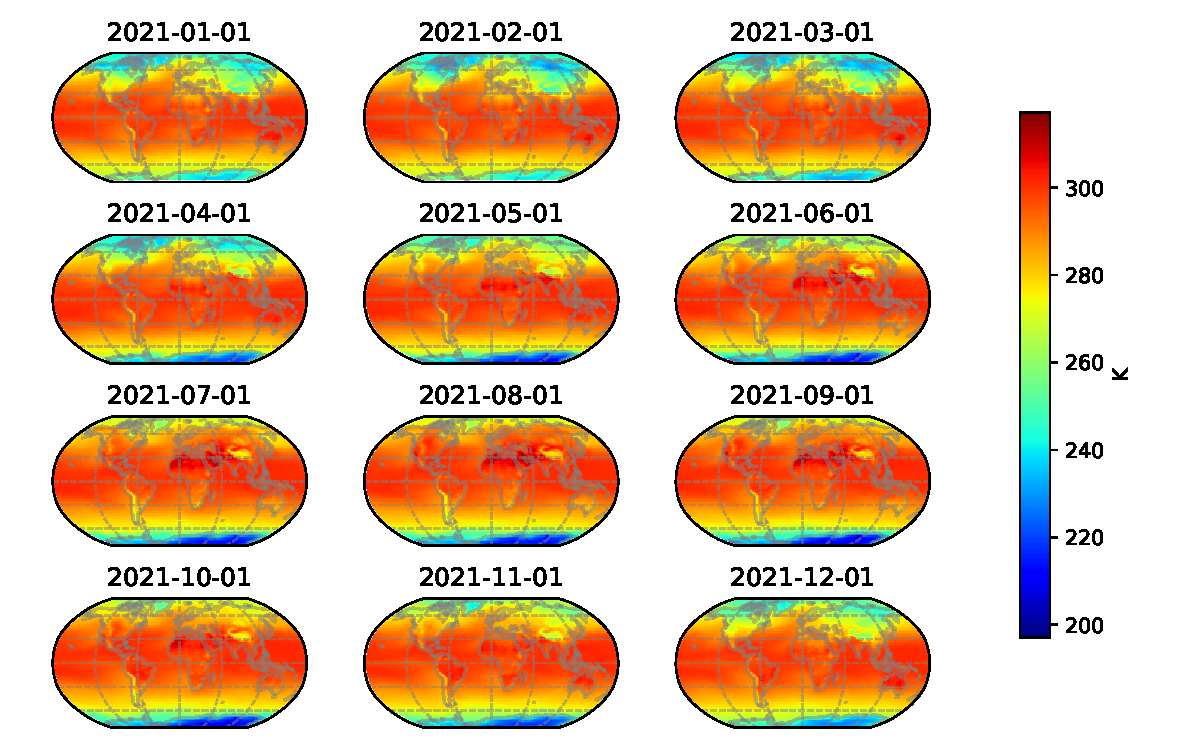
\includegraphics[width=1.0\textwidth]{cesm_temp_example}
	\caption[Average monthly temperature from CESM-LE]{Monthly average temperature over the globe in Kelvin ($\si{\kelvin}$) from a single simulation from CESM-LE. The figure illustrates both the temporal and spatial dependency that is observed in temperature across the globe. The figure is projected to the Robinson projection for illustration purposes.}
	\label{fig:cesm_example}
\end{figure}

The CESM data is generated through simulations of a complex model of the Earth (see Section~\ref{sec:cesmle} for more detail).
However, EO data is also becoming more frequently generated through remote sensing.
Remote sensing is the monitoring of a physical characteristic of an area through measuring its reflected and emitted radiation at a distance. 
Space borne remote sensing, typically achieved through the use of satellite based sensors, is becoming more prominent as a source of EO data and in particular as a source of climatology data.
The three studies above, \citep{muro_short-term_2016, raspini_continuous_2018, khabbazan_crop_2019}, use space borne remote sensing to observe their process of interest. 
This is largely due to the increase in satellites launched which have been designed to capture various processes of the earth.
Figure~\ref{fig:sar_timeline} highlights the rise in availability of a single type of remote sensing satellite.
One particularly prominent remote sensing system is the European Space Agency's Sentinel Constellation, \cite{aschbacher_european_2012}.
The Sentinel constellation of satellites provides a wide range of remote sensing sensors which are easily accessible.
The constellation provides capabilities to capture various physical characteristics through the many forms of sensors equipped to its satellites.
These include  Synthetic Aperture Radar (SAR), optical and multispectral sensors.
For example, European Space Agency's Sentinel-4 from the Sentinel Constellation, \cite{aschbacher_european_2012}, provides observation dedicated to air quality monitoring.
As such the Sentinel constellation has been widely used in EO studies; the three studies above, \citep{muro_short-term_2016, khabbazan_crop_2019, raspini_continuous_2018}  all utilise the Sentinel 1 SAR sensors for their observation source. 

\begin{figure}[htbp!] 
	\centering    
	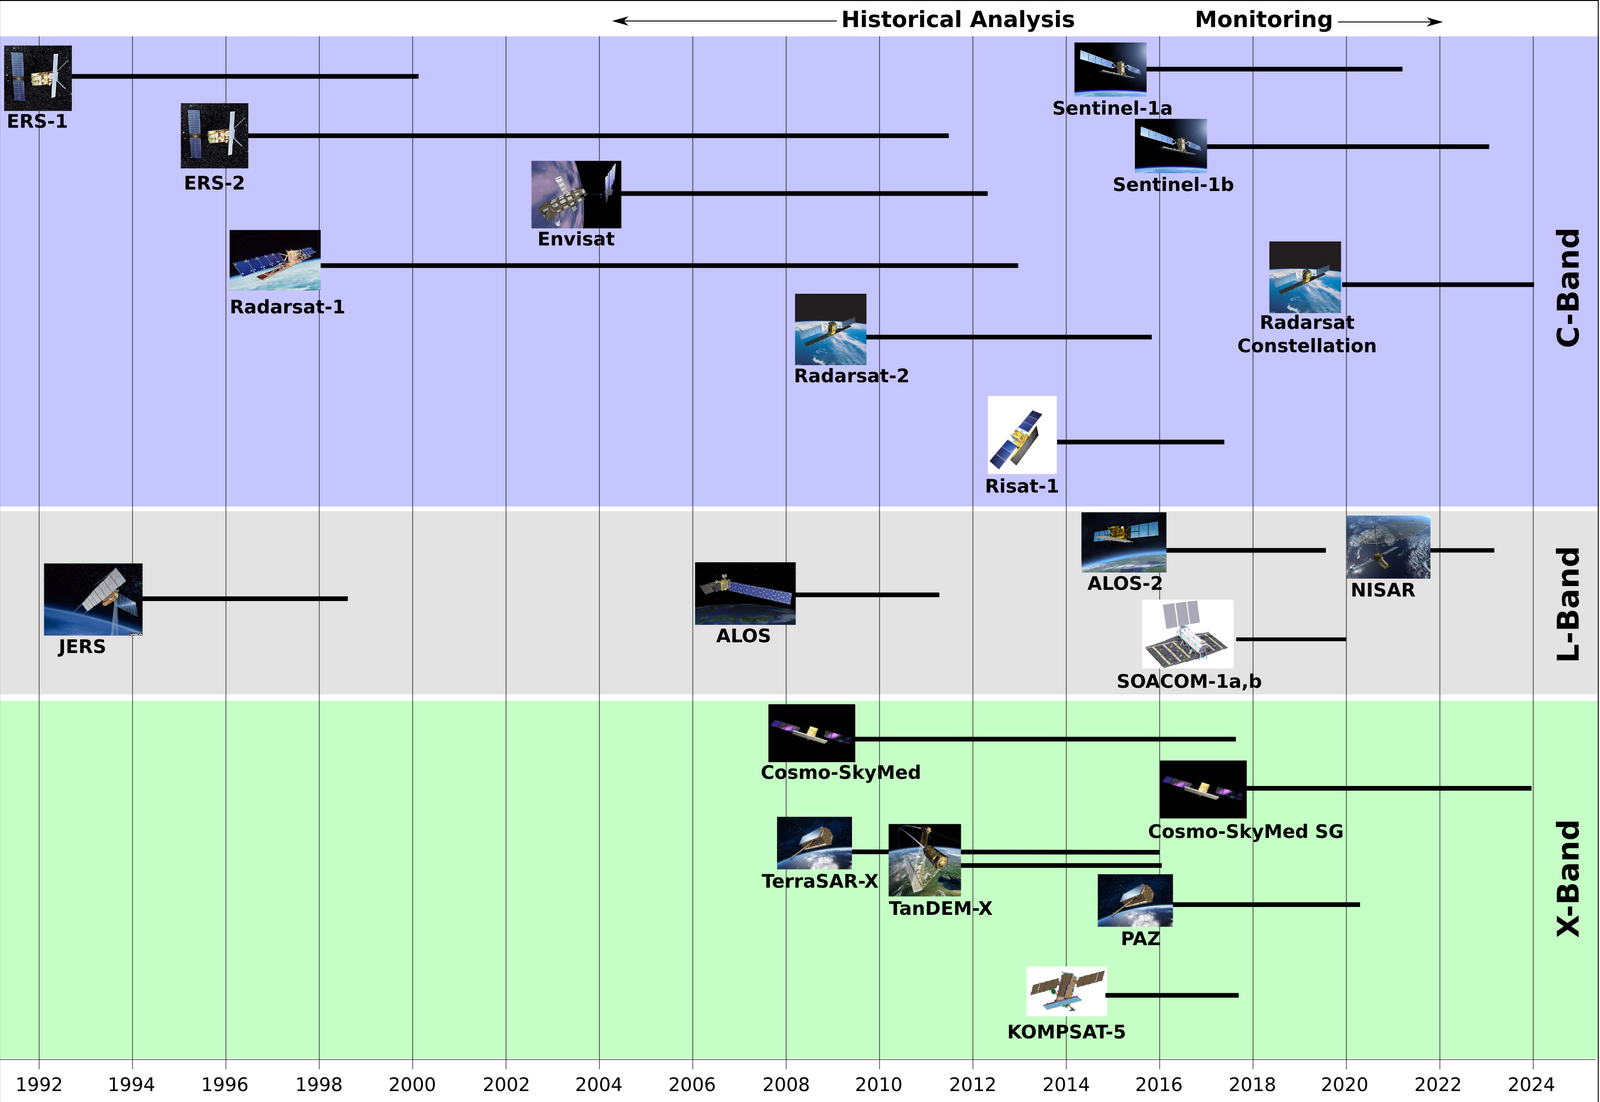
\includegraphics[width=1.0\textwidth]{Sensors}
	\caption[Timeline of major EO satellites]{A timeline of major satellite launches and operating periods for EO missions using SAR based sensors. This highlights the rapid rise in availability of such remote sensing capabilities, driven by the demand for observations to cover large spatial and temporal scales in areas such a climatology. The C, L, X band refers to the type of SAR sensor equipped to the satellite which are used in different applications. See \citep{oliver_understanding_2004} for details.}
	\label{fig:sar_timeline}
\end{figure}

A prominent focus of the Sentinel satellite constellation is to provide repeated observations at relatively high frequency, \cite{aschbacher_european_2012}.
This is in response to the rising demand for monitoring EO processes over time.
High frequency revisit times has been made possible by the development of remote sensing technologies.
For example, the Sentinel 1 satellite constellation can provide revisit times of approximately five days for areas of Europe.
Such short revisit times are advantageous as they give higher temporal resolution and thus studies can incorporate this additional information.
For example, \citeauthor{raspini_continuous_2018} utilise this in their study of land deformation change to identify anomalous regions, \citep{raspini_continuous_2018}.
The increasing availability of high temporal frequency EO data such as those provided by the CESM-LE data set or the Sentinel satellite constellation thus drives a demand for statistical models which can handle both high resolution spatial and temporal dependency.  

Earth observation data, such as those provided by the CESM model or through remote sensing, have an inherent spatial and temporal dependency.
That is to say the underlying process driving both remotely sensed observations of the Earth and the CESM simulations will vary over the globe and also will be driven by the state of the system at prior time points.
That is not to say the process is the same for both but rather that there is a commonality in that they could both be considered spatio-temporal processes.
In addition there are more concrete similarities in the collection of such EO data.
Typically, EO data are described on a lattice of points over space which is usually regular.
This usually relates to the pixels of an image over the area of interest.
Such a lattice is represented through a geodetic coordinate system which grounds a datum to a real world location.
Finally, EO data typically have repeated observations through time over the same space.
This usually relates to the repeated imaging of the same area of interest at multiple points in time.

The description of such spatio-temporal processes is well studied in statistics and a large amount of effort has been used to develop various models to suit them.
A well known monograph which deals with such processes is that written by \citeauthor{cressie_statistics_2011}, \cite{cressie_statistics_2011}.
The monograph details various forms of spatio-temporal processes and typically focuses on the extension of spatial method to incorporate the additional temporal dimension.
We discuss these methods in more detail in Section~\ref{sec:st_methods}.
Of particular importance in these methods is that temporal and spatial dimensions are treated distinctly as they are inherently different in the physical process.
For example, one could consider a spatial point influencing its neighbours in all directions however a temporal point reasonably shouldn't influence its past.
As such there is often a distinction in the method used to model the temporal and spatial aspects of the physical process.

An area of statistics which is often used to model data with temporal dependency is Functional Data Analysis (FDA).
FDA is typically applied to analyse data which vary over a continuum, \citep{ramsay_functional_2010}.
Time is one such continuum.
EO data with high frequency temporal observations are therefore suitable candidates for FDA models.
FDA is a relatively new branch of statistics and as such few studies have been presented which use FDA techniques on EO data.
\citeauthor{liu_functional_2012} consider FDA techniques on periodic EO data, \citep{liu_functional_2012}. 
Similarly \citeauthor{hooker_maximal_2015} consider FDA techniques to model the Harvard modified vegetation index sourced from EO data.
In both the above studies they consider EO data as a collection of functional observations indexed by space where each functional observation represents a trajectory over time.

The monograph of \citeauthor{ramsay_functional_2010} provides a comprehensive introduction to the themes of FDA, \citep{ramsay_functional_2010}.
FDA are often intuitive since viewing responses as being trajectories from an unknown smooth random function in some contexts closely matches the actual data generating process compared to a multivariate analysis.
The use of such techniques therefore could be helpful in modelling such high frequency EO data in conjunction with the multivariate methods discussed by \citeauthor{cressie_statistics_2011} in \citep{cressie_statistics_2011}.
However, focus in the FDA literature to date has primarily revolved around independently observed functional data.
This is typically not the case in our motivating case of EO data where there is often obvious spatial dependency.
Thus there is a need to describe functional data models which incorporate dependency among observations.
In this work we consider developing such models for dependent functional data with a focus on application to EO data.
We consider adapting well studied FDA methodologies and borrow techniques from spatio-temporal statistics to allow for spatially dependent observations.
In Section~\ref{sec:fr} we make concrete our definition of functional data. 

\section{Functional Representation \label{sec:fr}}
As mentioned in Section~\ref{sec:eo} EO data can be viewed as a collection of functional data.
However, there is a choice about how we interpret observations in this conversion.
We may consider the data as a collection of functional observations with time being our functional dimension and space our collection dimension.
For example, we may consider each spatial location from Figure~\ref{fig:cesm_example} giving rise to a trajectory over time of which we have only observed 12 time points.
Or we may consider the functional observations having a spatial domain and the collection dimension being time.
That is we may consider each image in Figure~\ref{fig:cesm_example} being a surface with observations only at pixel locations and the collection consists of a time series of such surfaces. 
The canonical presentation of functional data in FDA is to use time as the functional dimension, \citep{ramsay_functional_2010}, and thus we use the below definition of functional data from this point of view. 

\subsection{Functional data \label{ssec:fd}}
Multivariate data analysis usually revolves around the study of observations which are finite dimensional and is well studied.
Modern data collection techniques can now create data which are extremely numerous and thus can often be viewed as functions.

For example, \citeauthor{ferraty_nonparametric_2006} consider the case where we can observe a random variable at several times between some minimum and maximum time, $\left( t_{\text{min}}, t_{\text{max}} \right)$, \citep{ferraty_nonparametric_2006}.
A single observation can then be considered as the collection $ \{ X(t_j) ; j=1,2,\dots, J\}$ where $J$ is the total number of temporal sample points and $X(t)$ is the response variable at time $t$.
Unlike multivariate data we consider the case that the separation between observations becomes minimal.
That is we consider the data as an observation from the continuous random process $\mathcal{X} = \{X(t); t \in \left( t_\text{min}, t_\text{max} \right)\}$.
We therefore propose as in \citep{ferraty_nonparametric_2006} and \citep{shi_gaussian_2011} the following definition of a \textit{functional variable}.

 \begin{definition}[Functional Variable]
	A random variable $\mathcal{X}$ is called a functional variable if it takes values in an infinite dimensional space (or functional space). Observations $\chi$ of $\mathcal{X}$ are called a functional data.
	\label{def:functional_variable}
\end{definition}

Further to this, suppose we observe a collection of functional data (realisations of $\mathcal{X}$).
Then we will denote this collection by the term \textit{functional dataset}.

\begin{definition}[Functional Dataset]
	A functional dataset, $\chi_1, \chi_2, \cdots, \chi_N$ is the collection of $N$ realisations of functional variables $\mathcal{X}_1, \cdots, \mathcal{X}_N$ identically distributed to $\mathcal{X}$.
	\label{def:functional_dataset}
\end{definition}

The canonical way to present functional data and the subsequent methods is to use time as the continuous variable, \cite{ramsay_functional_2010, ferraty_nonparametric_2006, shi_gaussian_2011}, as described above.
However, there is no such restrictions in either Definition~\ref{def:functional_variable} or Definition~\ref{def:functional_dataset}. 
In fact, another case is to consider the functional domain of the variables to be space.
In our proposed methodologies we present when possible with respect to time due to the simplification it brings in notation.
We will make explicit reference to when we change the domain of our functional data, for example if we consider space as our continuous domain. 

We introduce the following notation for use in the remainder of this work.
We consider our EO data set to be observed in some spatial domain which we denote by $\mathcal{S} \subset \mathbb{R}^2$ and temporal domain donated by $\mathcal{T} \subset \mathbb{R}$.
Any observed dataset we can enumerate with one index over the spatial location and the other indexing the temporal locations.

We assume our dataset is comprised of $N$ spatial locations and let $\ve{s}_i \in \mathcal{S}$ be the spatial location of the $i^\text{th}$ observed functional variable.
At each spatial location we suppose we observe $J_i$ temporal observations and denote by $t_{ij} \in \mathcal{T}$ the $j^\text{th}$ temporal observation of the $i^\text{th}$ functional variable.
Then our dataset can be summarised by $Y$ where:
\begin{equation}
	Y = \{ y_{ij}; i=1,2,\cdots,N, j=1,2, \cdots, J_i \}
	\label{eqn:observed_data}
\end{equation}
where $y_{ij}$ is the response value of the $i^\text{th}$ functional variable at time $t_{ij}$ observed with error.
That is we consider for each spatial location the discrete temporal observations being a sample from a realisation of a functional variable observed with error.
That is:
\begin{equation}
	y_{ij} = \chi_{i}\left( t_{ij} \right) + \varepsilon_{ij}
	\label{eqn:fd_temporal}
\end{equation}
where, as in Definition~\ref{def:functional_dataset}, $\chi_i$ is a realisation of functional variable $\mathcal{X}_i$ for $i=1,2,\cdots,N$.
We consider each functional variable as being identically distributed as $\mathcal{X}$.
As is common in most observation models, we assume that we observe data with error.
Typically one assumes that the error process $\{\varepsilon_{ij}; i=1,2,\cdots,N, j=1,2,\cdots,J_i\}$ is a white noise process with variance $\sigma_\varepsilon^2$. 

In this case one considers the modelling of the EO dataset by ensuring smoothness of some kind over the temporal domain via its functional data representation.
We can then consider building in spatial dependency by assuming a sampling correlation in our $N$ functional data.
An area where such spatial dependency has been long studied is multivariate spatio-temporal methods.

\section{Spatio-Temporal Methods, \label{sec:st_methods}}
In the statistical literature spatial and spatio-temporal models have been extremely well studied, especially due to the prevalence of geo-statistical applications.
In the following we briefly review some of the most commonly observed spatial and spatio-temporal statistical models in the multivariate analysis literature. 

The monograph of \cite{cressie_statistics_2015} and references within provide a succinct summary of traditional methodologies in spatial statistics; many of which are applicable to EO data.
Generally speaking, spatial data can be split into one of three categories; geo-statistical, area, and point process data, \citep{cressie_statistics_2015}.
In this work the EO data described in Section~\ref{sec:eo}  are most suitably modelled using geo-statistical models.
The canonical model used in geo-statistical settings is the Kriging model.
The Kriging model is well described in \cite{stein_interpolation_1999}.
Such models treat spatial data as samples from a random spatial process and that predictions for unknown values can be calculated from a weighted combination of known values in a neighbourhood of our unknown location utilising the correlation among neighbouring points.
A prime example of the spatial Kriging model in use for EO data is given in \cite{rossi_kriging_1994}.
Extensions to the basic Kriging technique have also been employed across a number of geo-statistical settings, including Co-Kriging involving extra covariate information for reconstruction, \cite{zhang_restoration_2009}.
Kriging is well known in many fields through various names, in the FDA literature it is most often referred to as Gaussian processes regression.
\citeauthor{shi_gaussian_2011} describe in detail the concept of Gaussian processes in the context of functional regression, \citep{shi_gaussian_2011}, and we discuss them more in Section~\ref{sec:gp}. 

As is detailed in \cite{cressie_statistics_2015} a key aspect to geo-statistical modelling is the specification of spatial dependency in the observed data.
A common way for such specification is through parametric covariance or kernel functions.
Traditional stationary parametric functions such as the Mat\`{e}rn covariance are discussed in detail in \cite{cressie_statistics_2015}.
These commonly rely on the assumption of isotropy and stationarity in modelling which rarely holds in practice.
Further literature has considered extensions of these and is in fact an active area of research.
\citeauthor{schmidt_flexible_2020} compare a variety of methods for producing non stationary and heterogeneous covariance structures for the goal of spatial interpolation, \citep{schmidt_flexible_2020}.
They group the various methods of creating such structures into four categories; deformation, convolution, covariate, and stochastic partial differential equations.
The deformation approach proposed by \citeauthor{sampson_nonparametric_1992} extends the anisotropic stationary covariances, such as those described in \cite{cressie_statistics_2015}, by allowing for a non linear transformation to the space which creates a latent space where isotropy holds, \cite{sampson_nonparametric_1992}.
The convolution approach proposed by \citeauthor{higdon_space_2002} uses a specific form of the covariance kernel which can be represented as a convolution between a convolution kernel and a white noise process.
We discuss such an approach more in Chapter~\ref{cha:cpace}.
The covariate based approach to constructing non stationary kernels tends to use an adaption to the convolution or deformation approaches with specific covariates, \citep{schmidt_flexible_2020}.
Finally the stochastic partial differential equation method proposed by \citeauthor{lindgren_explicit_2011} construct non stationary covariances through formulating the resulting Gaussian process as the solution of a stochastic partial differential equation which guarantees the construction of a well defined covariance function, \citep{lindgren_explicit_2011}. 

A natural extension to purely spatial modelling of spatio-temporal data is to include the temporal domain.
Such models are known as spatio-temporal models.
Spatio-temporal models are well discussed in the monograph \cite{cressie_statistics_2011} by \citeauthor{cressie_statistics_2011}.
Spatio-temporal Kriging models are well suited to EO data; however these models are relatively scarce in the literature.
\citeauthor{militino_introduction_2018} considers the application of such modelling in the satellite remote sensing literature and reasons the lack of them is primarily due to the added complexity these models produce in specifying valid space-time covariance functions, \cite{militino_introduction_2018}.
As such, one particular direction spatio-temporal modelling has considered is the creation of spatio-temporal covariance functions.
Spatio-temporal covariance functions are discussed in \citep{cressie_statistics_2011}.
Separability between spatial and temporal correlations is often a key assumption in some methods due to the reduction in computational complexity they provide.
The separability assumption proposes that a space-time covariance function $k(\ve{s}, t, \ve{s}^\prime, t^\prime)$ can be factored into two separate covariance functions $k_{s}(\ve{s}, \ve{s}^\prime)$ and $k_t(t, t^\prime)$, one for each of the spatial and temporal dimensions. 
In particular for EO data, \cite{george_selecting_2015} consider the selection of separable covariances and \cite{deb_spatio-temporal_2019} consider such models for air pollution data. 
However, the separability assumption may be too restrictive for capturing complex spatio-temporal processes, \citep{cressie_statistics_2011}. 
As such \citep{mitchell_likelihood_2006, fuentes_testing_2006, aston_tests_2017} considers tests for when the separability assumptions hold.
The work in \citep{cressie_classes_1999, gneiting_nonseparable_2002, iaco_nonseparable_2002} consider the construction of non separable covariance functions for when separability doesn't hold for use in spatio-temporal models.

\section{\label{sec:summary_research}Summary of Research}
The motivation of this work is to provide a model designed for EO data which provides an explanation of both the spatial and temporal process in a parsimonious way.
We present a novel method named Correlated Principal Analysis through Conditional Expectation (CPACE), that is designed for modelling EO data.
The model builds upon existing FDA techniques to extend modelling from independently observed functional data to functional data which exhibits spatial correlation.
The emphasis in this work is to utilise the FDA paradigm over the temporal domain to aid in the decomposition of the data; with the understanding that our data generating process is smooth across the temporal domain.
Such a decomposition gives a parsimonious description of the data with respect to its temporal domain by describing its principal modes of variation.
We then estimate a spatial correlation structure for each component using well known spatial statistical methods.
The combination of the resulting estimated spatial covariance structures with the principal directions aims to capture the majority of temporal and spatial dependency observed in the data.
We can then utilise the CPACE model to help predict responses at unseen spatial and temporal locations, which is an area of keen interest in EO studies.
We assess our model using various simulated data both with known correct data generating distribution and to simulations drawn from an incorrect data generating procedure.
We apply our CPACE model to selected atmospheric variables from the CESM data set as an example application of the model to EO data.

The work is structured as follows.
In Chapter~\ref{cha:data} we describe our example data sets which we use to illustrate the performance of the model.
In Chapter~\ref{cha:background} we present the methodologies underpinning the CPACE models, these are typically well known FDA and spatio-temporal statistical methods.
We also present the smoothing methodologies used to estimate the mean and covariance surfaces of our random functional variables.
In Chapter~\ref{cha:ftsm} we present an interim model built on the combination of two well known existing methodologies in the FDA literature with a focus on application to an EO data set.
Such a model proposes an novel approach to modelling EO data and helps to highlight the need of including both spatial and temporal effects in modelling such data.
In addition, the proposed model in Chapter~\ref{cha:ftsm} gives an opportunity to explore EO data where the functional domain is space rather than time.
We present the benefits and limitations of such an approach in practice in this chapter.
In Chapter~\ref{cha:cpace} we introduce the main contribution of this work; which is the CPACE model for correlated functional data.
We describe the model in detail as well as providing asymptotic results.
In Chapter~\ref{cha:application} we apply the CPACE model to simulated data and in Chapter~\ref{cha:real_application} to real world data sets.
Simulation results are presented with comparisons to various existing models with a focus on comparative ability to recover known data generating parameters.
Applied results to real world data sets are included with comparisons to existing techniques with a focus on interpolation and forecasting abilities of the model.
In Chapter~\ref{cha:implementation} we highlight the practical difficulties in implementing the model with discussion on various techniques which are used to overcome the high dimensionality which is typical in the EO data.
Finally, in Chapter~\ref{cha:conclusions} we draw the conclusions of the work and present area of further work. 